% Einleitung
\section{Basics}
\begin{minipage}{9cm}
\subsection{Euclidean Algorithm}
With the Euclidean Algorithm the $gcd$ is found on base of $gcd(a,b)=gcd(b,a \mod b)$ 
Pseudo code:
\begin{verbatim}
	int gcd(int a, int b){	=> a>b
		while(b \inq 0){
			r = a mod b
			a = b
			b = r
		}
		return a
	}
\end{verbatim}
The \em Extended Euclidean Algorithm \em return the $gcd(a,b)$ 
and how can it build out of $a,b$ $\Rightarrow gcd(a,b)=x a + y b$. 
e.g:\\ 
$gcd(78,99)=3=14 \cdot 78 - 11 \cdot 99$\\
\tr{eucl(a,b)}{$\{x\; y \; gcd(a,b)\}$}\negmedspace; $y=b^{-1} \mod a$\\
\tr{eucl(12,9)}{$\{1\, -\negmedspace 1 \quad 3\}$}$=12-9=3$\\
\end{minipage}
\hspace{4mm}
\begin{minipage}{9.5cm}
\subsection{Eulers Phi-Function $\varphi(n)$}
Sie gibt f\"ur jede nat\"urliche Zahl $n$ an, wie viele zu $n$ teilerfremde positve 
ganze Zahlen es gibt, die nicht gr\"osser als $n$ sind.\\
\tr{ephi(n)}{$\varphi(n)$}\\ 

\begin{tabular}{| l l l |}
	\hline
	1:		&	$n=p \to p=Primzahl(PZ)$				&	$\varphi(n)=p-1$\\
	2:		&	$n=p \cdot q \to p,q=PZ$	&	$\varphi(n)=(p-1)(q-1)$\\
	3:		&	$n=p^k \to p=PZ$			&	$\varphi(n)=p^k-p^{k-1}$\\
	\hline
\end{tabular}

\subsection{Modulare Arithmetic}
$a \equiv b \mod m$ and $c \equiv d \mod m \to a=b+k \cdot m$; $k \in \mathbb{N}$ \\
\begin{liste}

\item $a \cdot c \mod m = (a \mod m) \cdot (c \mod m) \Rightarrow$ \\ Reduktion durch kleinere Zahlen
\item $a + b \mod m \equiv b \mod m + d \mod m$
\item $k a \equiv k b \mod m$
\end{liste}
\end{minipage}
\subsection{Modulares Inverses}
Definition: $a \cdot x \equiv 1 \mod m \Rightarrow x \equiv a^{-1} \mod m$\\
Tatsache: $x$ existiert genau, wenn $gcd(a,m)=1$\\
Trick: $1 = a \cdot x + m \cdot y \Rightarrow 1 \equiv a \cdot x \mod m$ (use \em Extended Euclid (a,m) \em)\\
BSP: $a = 16, m = 13; a^{-1} \mod m \equiv 5$ \\
\tr{inv(a,m)}{$a^{-1}$}

\subsection{Fermat's little Theorem}
\begin{tabular}{l l}
	$p$=prime number					&	if $\alpha$ and $p$ are coprime (coprime = Teilerfremd = $gcd(\alpha,p)=1$)\\
	$\alpha^p \equiv \alpha \mod p$		&	$\alpha^{p-1} \equiv 1 \mod p$ e.g. \\
	$a=3; p=7$ 							&   $3^6 \mod 7 \equiv 1 \mod 7$ \\\\
   $\bm{\alpha^{\varphi(m)} \equiv 1 \mod m}$  & $\Rightarrow$ if $\alpha$ and $m$ are coprime. e.g\\
   $m=15\Rightarrow\varphi(15)=\varphi(3\cdot5)=(3-1)(5-1)=8$ &  $\Rightarrow a^8\equiv 1 \mod 15$\\
\end{tabular}\\\\
Note: Fermat's little Theorem does only give an upper bond for the exponent $e$ such that $\alpha^e=1\mod p$. For some
integers $\alpha$, there may exist an exponet $e<p-1$ such as $\alpha^e \equiv 1 \mod p$.\\


\subsection{Order of Elements}
$g \in \mathbb{Z}, \quad e \in \mathbb{N}, \quad p \in \mathbb{N} \rightarrow$ kleinste Zahl $e$ sodass \boxed{g^e \equiv 1 \mod p} gibt die
Ordnung von $g \mod p$.\\
$g^n \mod m \equiv 1 $ wenn $n=k\cdot e$\\
$g^l = g^k$ wenn $l\equiv k \mod e$\\ 
$\beta = g^i \mod p \Rightarrow \beta =$ Generator modulo p wenn $gcd(p-1,i)=1$ (coprime)\\
$g$ ist Generator modulo $p$, falls $g^i;1 \leq i \leq p-1$ die Zahlen $\{1,\ldots,p-1\}$ erzeugt. \\
Equivalent gilt: $g$ ist ein Generator modulo $p$, falls die Ordnung von $g\mod p$ gleich $p-1$ ist (also $e=p-1$).\\
Die Anzahl Generatoren modulo $p$ berechnet sich mit $\varphi(p-1)$

\subsection{Chinese Remainder Theorem}
Wird verwendet um ein Gleichungssystem zu l\"osen: \\
\begin{minipage}{4cm}
$x \equiv a_1 \mod m_1$\\
$x \equiv a_2 \mod m_2$\\
$\ldots$\\
$x \equiv a_n \mod m_n$\\
\end{minipage}
\begin{minipage}{14cm}
$m=\displaystyle\prod_{i=1}^{n} m_i, \quad M_i=m/m_i, \quad gcd(m_i, M_i)=1, 1 \leq i \leq n$\\
$y_iM_i \equiv 1 \mod m_i \to y_i\equiv M_i^{-1} \mod m_i \to$ \tr{eucl($M_i,m_i$)}{$\{.., y_i,.. \}$}, \\
$x=\left(\displaystyle\sum_{i=1}^{n} a_i  y_i M_i \right) \mod m=\left(\displaystyle\sum_{i=1}^{n} a_i  y_i M_i \right) \mod m $
\end{minipage}\\
\\
\begin{minipage}{5cm}
Beispiel:\\
$x\equiv a_1 \mod m_1 = 5  \mod 7$\\
$x\equiv a_1 \mod m_1 = 3  \mod 11$\\
$x\equiv a_1 \mod m_1 = 10 \mod 13$\\
$x=?$
\end{minipage}
\begin{minipage}{5cm}
$m=m_1 m_2 m_3 = 7\cdot 11 \cdot 13 = 1001$\\
$M_1=m/m_1=11 \cdot 13 = 143$\\
$M_2=m/m_2=7 \cdot 13 = 91$\\
$M_3=m/m_3=7 \cdot 11 = 77$\\
\end{minipage}
\begin{minipage}{8cm}
Mit extended euclid: (e.g. $y_1=exteucl(M_1,m_1)$)\\
$y_1=5;  y_2=4; y_3=12$; $M_1 y_1 \equiv 1 \mod m_1$\\
$\bm x\equiv a_1\cdot y_1\cdot M_1+a_2\cdot y_2\cdot M_2+a_3\cdot y_3\cdot M_3 (\mod m)$\\
$\bm x\equiv 5\cdot5\cdot143+3\cdot4\cdot91+10\cdot12\cdot77 \equiv \bm{894} \mod 1001$\\
Check $\Rightarrow 894 \mod 7 \equiv 5; \quad 894 \mod 11 \equiv 3;$ etc.
\end{minipage}

\subsection{Faster Exponentiation: Square and Multiply}
Um den Modulos von grossen Potenzen zu rechnen werden die Potenzen in Zweierpotenzen heruntergebrochen und Schritt für Schritt ausgerechnet:\\
$g^e=g^{\sum c_i 2^i}=\prod_{i=0}^k \left(g^{2^i}\right)^{e_i}=g^{e_0}\cdot\left(g^{e_1}\left(...\left(g^{e_{n-1}}\left(g^{e_n}\right)^2\right)^2...\right)^2\right)^2$
\begin{aufzaehlung}
\item Drücke die gegebene Potenz in Zweierpotenzen aus: $e=73=2^0+2^3+2^6$
\item Berechne die Zweierpotenzen $g^{2^i} \mod m$ und reduziere nach jeder Berechnung: $g=6\Rightarrow$\\ 
$6^{2^1} \mod 100 = 36;\quad 6^{2^2} \mod 100 \equiv 36^2  \mod 100 \equiv 96;\quad  6^{2^3} \mod 100 \equiv {-4}^2 \mod 100 \equiv 16; \ldots$
\item Berechne das Produkt der Zweierpotenzen: $6^{2^0}\cdot6^{2^3}\cdot6^{2^6}\mod 100\equiv 36 \cdot 16 \cdot -4 \equiv 16\mod 100$
\end{aufzaehlung}
Mit Hilfe des \em Square and Multiply \em wird der Rechenaufwand auf $\log_2(e)$ Potenzen und auf $1/2 \log_2(e)$ Multiplikationen reduziert. \\
Falls man beim Berechnen der Zweierpotenzen an die Grenzen des Rechner stösst, dann kann man die Potenz unterteilen und in zwei Schritte berechnen 
(Bsp. $6^{2^{10}}=(6^{32})^{32} \mod 100$).

\subsection{Glossar}
\begin{minipage}{12.5cm}
\begin{tabular}[]{|l |p{9cm}| }
	\hline
	bijektiv			&	umkehrbar eindeutig		\\
	\hline
	injektiv			&	Sie besagt, dass jedes Element der Zielmenge $Y$ einaml als Funktionswert angenommen wird.
							Es werden also keine zwei verschiedenen Elemente der Definitionsmenge $X$ auf dasselbe Element in 
							der Zielmenge $Y$ abgebildet.		\\
	\hline
	permutation			&	(Vertauschen) versteht man die Ver\"anderung der Anordnung von Objekten in einer Reihenfolge
							durch Vertauschen der Elemente.			\\
	\hline
	affine Abbildung	&	lineare Abbildung, es bleibt Kolinearit\"at, Parallelit\"at und Teilerverh\"altnisse erhalten.	 \\
	
	\hline
\end{tabular}\\

\end{minipage}
\begin{minipage}{6cm}
\textbf{Irreduzible Polynome in:}\\
\begin{tabular}{l l}
	$GF(2)$				&	$GF(3)$\\
	\hline
	$x$					&	$x^2+1$\\
	$x+1$				&	$x^2+x-1$\\
	$x^2+x+1$			&	$x^2-x-1$\\
	$x^3+x+1$			&	$x^3-x+1$\\
	$x^3+x^2+1$			&	$x^3-x-1$\\
	$x^4+x+1$			&	$x^3+x^2+x-1$\\
	$x^4+x^3+1$			&	$x^3+x^2-x+1$\\
	$x^4+x^3+x^2+x+1$	&	$x^3+x^2-1$\\ 
						&	$x^3-x^2+1$\\ 
						&	$x^3-x^2+x+1$\\ 
						&	$x^3-x^2-x-1$\\ 
\end{tabular}
\end{minipage} \\

\subsection{Polynom division}
\begin{minipage}{10.5cm}
	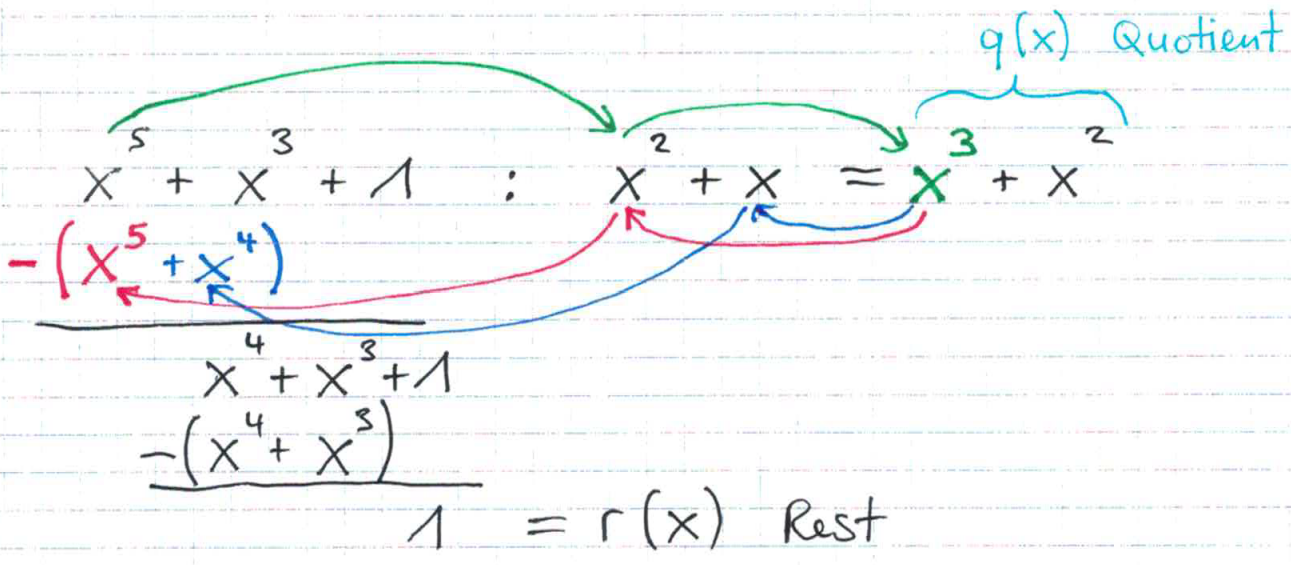
\includegraphics[width=10cm]{./bilder/polynomdivision.png}\\
\end{minipage}
\begin{minipage}{8cm}
	Polynom division can be used to determine whether a given polynomial is irreducible or not, i.e. if the division with any other polynomial (up to the half 
	order of the dividend polynomial) has a rest $r(X)$ or not. In this example, the calculation is done in $GF(2)$, meaning that negative values are 
	equivalent to positive values. In this case $r(X)\neq 0$ and the given polynomial is irreducible.\\
	A polynomial that is not divisible by any polynomial of degree 1 and 2, is also not divisible by any polynomial of higher degree, because a factorization 
	would yield a divisor of degree 1 or 2, respectively.\\
\end{minipage}


